\documentclass{amsart}
\usepackage{amsmath}
\usepackage{graphicx}
\title{Bayesian modeling of COVID-19 epidemic: Japanese case}
\author{Yoriyuki Yamagata}
\address{National Institute of Advanced Industrial Science and Technology (AIST),
1-8-31 Midorigaoka, Ikeda, Japan}
\email{yoriyuki.yamagata@aist.go.jp}
\date{\today}

\begin{document}

\maketitle

\begin{abstract}
 We estimate the daily change of a ``contact frequency'' and reporting rate in Japan by a Bayesian method.
 The estimate reveals a recent downward trend.
 Although our analysis is preliminary, this may suggest that Japanese policy had some impact on the spread of infection.
\end{abstract}

\section{Introduction}

In the wake of the COVID-19 epidemic, the Japanese government gradually employed public health measures against COVID-19.
In the first stage, the stronger quarantine measures at the border were implemented.
Once patients who had no connection to Wuhan appeared inside the border, The government started to track these patients as far as possible and tried to find people contacted to these patients.
Once these ``track and quarantine clusters'' tactics were overwhelmed by the number of patients, the government started to ask ``behavior changes'' to people, culminating ``declaration of the emergency'' on April 6.
Public facilities like libraries were closed.
Large shopping malls and entertainment businesses, such as movie theatres, were asked to be closed.
Restaurants are asked to shorten their operating hours and stop providing alcoholic beverages at night.
Working from home was encouraged, and the citizens were advised to avoid crowded areas and generally avoid going outside unnecessarily.

However, the Japanese legal system does not have enough mechanisms to ``enforce'' these policies.
Thus the effectiveness of these policies is questionable.
Many people are still commuting to their office because many companies lack the necessary ability to allow their employees to work from home.
Many small restaurants and cafes are still running their business because of the lack of financial compensation.

In this paper, we apply a Bayesian method to estimate daily changes of a ``contact parameter'', which determines the speed of infection, and reporting rate.
The result revealed a recent downward trend of the ``contact frequency''.
Thus, although our analysis is preliminary, this may indicate that Japanese policy has some effect against COVID-19 infection.
However, the reduction of ``contact frequency'' only reaches the level of the minimum achieved around mid-March, thus it would not be sufficient to prevent the spread of infection yet.

\section{Related works}

Several works employ data-driven methods to predict and measure the public health measure of COVID-19.

Anastassopoulou et al.~\cite{Anastassopoulou2020} apply the SIRD model to Chinese official statistics, estimating parameters using linear regression.
The reporting rate is not estimated from data but assumed.
By these models and parameters, they predict the COVID-19 epidemic in Hubei province.

Diego Caccavo~\cite{Caccavo2020} and independently Peter Turchin~\cite{Turchin2020} apply modified SIRD models, in which parameters change overtime following specific function forms.
Parameters govern these functions are estimated by minimizing the sum-of-square-error.
However, using the sum-of-square method causes over-fitting and always favors a complex model, therefore it is not suitable to access policy effectiveness.
Further, fitting the SIRD model in the early stage of infection is difficult, as pointed out in stat-exchange~\footnote{https://stats.stackexchange.com/questions/446712/fitting-sir-model-with-2019-ncov-data-doesnt-conververge}.
Using a Bayesian method, we avoid these problems to some degree, because a Bayesian method estimates parameter distribution instead of the point estimate.
Thus, we can assess the degree of confidence of each parameter.
Further, by well-established statistical methods, we can compare the explanatory power of different models.

Flaxman et al.~\cite{Flaxman2020} use a Bayesian model to estimate policy effectiveness.
The methodology is different from us because they assume immediate effects from the policies implemented.
Further, they use a discrete renewal process, a more advanced model than the SIRD model.
They use parameters estimated from studies of clinical cases while we use a purely data-driven method.

\section{Method and materials}

\subsection{Model}

We use the well-known SIRD model but make some modifications.
Bayesian estimation requires a large number of simulation runs, so solving ordinary differential equations is too computationally expensive.
Therefore, we replace ordinary differential equations to difference equations.
However, this causes numerical instability.
To mitigate instability, we split $\beta$ in SIRD model into a ``contact frequency'' $b$ and infection probability $p$.
Let $S$ be the number of susceptible people, $I$ that of infected people, $D$ that of death and $P$ population.
The probability of that one susceptible individual will be infected for each time step is estimated by $1 - (1 - p)^{b I / (P - D)}$.
We can introduce the ``quarantine measure'' $\alpha$, which indicates the ratio of interaction between infected people and uninfected people, as $1 - (1 - p)^{b \alpha I / (P - D)}$.
However, this cannot be distinguished by the equation above, so we use $1 - (1 - p)^{b I / (P - D)}$ as a probability.
Then, the average number of new infection is $S \cdot \{1 - (1 - p)^{b I / (P - D)} \}$.
Further, the process is stochastic, therefore 

\begin{align}
 NI(t) &\sim \textup{Poisson}(S \cdot \{1 - (1 - p)^{b I / (P - D)} \})\\
 NR(t) &\sim \textup{Poisson}(\gamma I)\\
 ND(t) &\sim \textup{Poisson}(\delta I)\\
 I(t+1) &= I(t) + NI(t) - NR(t) - ND(t)\\
 S(t+1) &= S(t) - NI(t)\\
 R(t+1) &= R(t) + NR(t)\\
 D(t+1) &= D(t) + ND(t)
\end{align}

We cannot expect that these values are directly observable, because many (or most) cases are mild or asymptomatic.
Therefore, we introduce the reporting rate $q$ and let the number of cumulative observed cases $C_{\text{obs}}$, recovered $R_{\text{obs}}$ and death $D_{\text{obs}}$ as
\begin{align}
 NI_{\text{obs}}(t+1) &\sim \textup{Poisson}(q * NI(t))\\
 NR_{\text{obs}}(t+1) &\sim \textup{Poisson}(\gamma * I_{\text{obs}}(t))\\
 ND_{\text{obs}}(t+1) &\sim \textup{Poisson}(\delta * I_{\text{obs}}(t))\\
 I_{\text{obs}}(t+1) &= I_{\text{obs}}(t) + NI_{\text{obs}}(t+1) - NR_{\text{obs}}(t+1) - ND_{\text{obs}}(t+1)\\
 R_{\text{obs}}(t+1) &= R_{\text{obs}}(t) + NR_{\text{obs}}(t)\\
 D_{\text{obs}}(t+1) &= D_{\text{obs}}(t) + ND_{\text{obs}}(t)
\end{align}

We assume that $b$ and $q$ change day to day bases while other parameters are fixed.
To get a reasonable estimate, we assume prior distributions somewhat arbitrary chosen.
\begin{gather}
 S(0) = I(0) \sim \textup{Gamma}(1, 1)\\
 b(0) \sim \textup{Gamma}(1, 1)\\
 q(0) \sim \textup{Beta}(1, 1)\\
 b(t+1) \sim \textup{Gamma}(b(t), 1)\\
 q(t+1) \sim \textup{Beta}(q(t), 1-q(t))
\end{gather}

% \subsection{Implementation}

% We used Stan~\cite{carpenter2017stan} for Bayesian modeling and parameter inference.
% Inferred data was processed ArviZ~\cite{arviz_2019}.
% Pandas~\cite{reback2020pandas} and xarray~\cite{hoyer2017xarray} were used for pre- and post-data processing.
% Seaborn~\footnote{https://seaborn.pydata.org} was used for visualization.

\subsection{Experiment}

Data up to April 18 were drawn from data repository~\footnote{https://github.com/CSSEGISandData/COVID-19} by Johns Hopkins University Center for Systems Science and Engineering.
Nation-wide numbers of confirmed cases, recovered cases and death were obtained.

These data were fed to Stan~\cite{carpenter2017stan} for Bayesian modeling and parameter inference.
We simplified our model to easy modeling in Stan.
Because latent discrete variables cannot be used in Stan, we used real numbers for $NI(t), NR(t)$ and $ND(t)$.
We used normal approximation $\mathcal{N}(\lambda, \sqrt{\lambda})$ for the Poisson distribution used for $NI(t)$.
For $NR(t)$ and $ND(t)$, we replaced stochastic laws to deterministic laws
\begin{align}
 NR(t) &= \gamma I\\
 ND(t) &= \delta I
\end{align}
to avoid a numerical issue.

Parameter estimation used 100,000 iterations with 50,000 iterations for warm-up and 50,000 iterations for sampling.
Four (default number of Stan) independent computations were performed simultaneously and used to check convergence.
$\hat{R}$~\cite{vehtari2019rank}, which measures convergence, were excellent, within $\hat{R} < 1.1$ for all parameters. 

To make sure that our results are meaningful, we compared the performance of our model with a model (we refer it by ``the constant model''), which assumes constant $b$ and $q$.
Parameters were estimated for the constant model in the same way and LOO-CV, a standard measure of model performance, was compared.
Because the exact computation of LOO-CV is computationally expensive, approximation PSIS-LOO-CV~\cite{Vehtari2017} is usually used.
Unfortunately, the assumption based on PSIS-LOO-CV seems broken for our case according to diagnostic messages due to high Pareto-k.
Therefore, we calculated LOO-CV directly by excluding data for a day, estimating parameters using the rest of the data and making a prediction of excluded data.
Averaging errors of a prediction, we can obtain the LOO-CV value.
The LOO-CV of our model was -2144.49497236, while the constant model was -2145.68817238. Therefore our model slightly outperformed the constant model.

Models and the computation history used for this experiment are public at GitHub~\footnote{https://github.com/yoriyuki/BayesianCOVID19/tree/start-writing-paper/notebook}.

\section{Results}

Fig.~\ref{fig:b} shows an estimated contact frequency for each day.
Because the Bayesian estimation gives a distribution of parameters, the lower (25\% percentile) estimate is shown by a dotted green line, the median estimate is shown by a solid blue line and the upper (75\% percentile) is shown a broken orange line.
\begin{figure}[h]
 \centering
 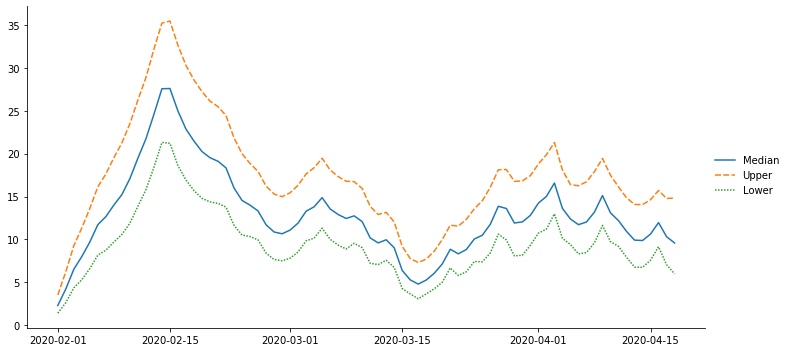
\includegraphics[width=\linewidth]{fig/b-Japan.png}
 \caption{ change over time of the contact frequency $b$}
 \label{fig:b}
\end{figure}
The upward trend until mid. February is probably an artifact of a prior used for $b(0)$, which is low compared estimated $b(t)$.
The downward trend until mid. March could be explained by public awareness and tracking effort of infection.
After mid. March, the tracking effort could be overwhelmed, thus created an upward trend until the beginning of April, when ``the state of emergency'' was declared to major urban areas.
Since then, there was a slow downward trend, but it is unclear how long it will continue.
It appears that ``the state of emergency'' only achieved the minimum contact frequency achieved around mid. March so far.
Interestingly, the result clearly shows a weekly cycle of the contact frequency peaked on Thursday.

\begin{figure}[h]
 \centering
 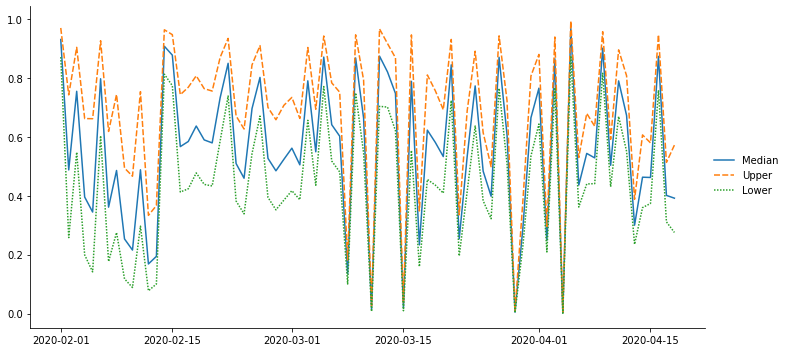
\includegraphics[width=\linewidth]{fig/q-Japan.png}
 \caption{Change over time of the reporting rate $q$}
 \label{fig:q}
\end{figure}

Fig.~\ref{fig:q} shows an estimated reporting rate.
The result is very noisy.
It could suggest that the reported number is strongly influenced by reporting practice.

\section{Discussion}

The universal applicability of our method is not clear.
The model was applied to Korean and Italian data.
However, the estimate did not converge in the case of Korea.
Traces of Markov Chain Monte Carlo, on which method Stan is based, revealed that one trace did not change from the initial value at all.
This would suggest a numerical problem in our model.
For the Italian case, the estimate converged except the death rate.
However, LOO-CV was worse than the constant model. Thus the result is not reliable.

There is a lot of room for improvement.
First, the sensitivity analysis of Bayesian priors would be required.
Also, the use of LOO-CV for model selection needs to be reconsidered because LOO-CV measures the model's prediction capability, but our goal is not a prediction.
Further, we need to analyze the reason for the divergence in the case of Korea.
Finally, we want to apply our method to more countries and compare the effectiveness of each country's policy. 

\bibliographystyle{plain}
\bibliography{BayesianCOVID-19}

\end{document}